\section{Übertragung des Saga-Patterns auf verteilte Transaktionen}

Das von \citeauthor{GarciaMolina.1987} vorgeschlagene Implementierungsmuster baut auf ACID-Transaktionen auf. Es wird davon ausgegangen, dass eine ACID-Transaktion sequentiell kleinere ACID-Transaktion aufgeteilt werden kann. Der Rollback-Mechanismus dieser Teiltransaktionen muss mittels zugehöriger Kompensierungen per Implementierung nachgebildet werden. In \cref{sec:section-garcia-paper} wurde erläutert, dass das Saga-Muster durch die Auflösung der Atomarität und Isolation und somit auch der Konsistenz keine strenge ACID-Sicherheit gewährleisten kann. 

\subsection{Saga-Patterns und BASE-Eigenschaft}
Da nun etabliert wurde, dass das Saga-Pattern grundsätzlich keine strenge ACID-Eigenschaften unterstützt, soll es mit dem alternativen Datenkonsistenzmodell BASE vergleichen werden, da sie sich sehr ähneln. Die Rollback-Logik des Saga-Patterns ist eine Möglichkeit mit \textit{Soft State} umzugehen. Das Aufbrechen der LLT in Teiloperationen ist im BASE-Modell ebenfalls vorhanden, da Veränderungen über mehrere Aggregate nicht atomar sind. Auch das Interesse des Saga-Patterns an Hochverfügbarkeit ist im BASE-Modell als \textit{Basically Available} zu finden. 

\textbf{Das Saga-Pattern kann also als eine Implementierung des BASE-Modells aufgefasst werden.}

\subsection{Anwendung des Patterns auf verteilte Transaktionen}
Das Paper \citetitle{GarciaMolina.1987} befasst sich mit dem Saga-Pattern als Implementierungswerkzeug innerhalb eines zentralen Systems. Die ACID-Eigenschaft wurde lediglich aufgelöst, um das blockierende Verhalten zu umgehen und Hochverfügbarkeit zu erreichen. 

Ein verteiltes System stellt sich dem selben Problem. Die Daten eines verteilten Systems sind über mehrere Datenbanken verteilt. Der Zugriff auf diese Daten ist häufig nur über einen dazugehörigen Microservice möglich. Muss also eine LLT Operationen in mehreren Datenbanken durchführen, dann kann das Saga-Pattern auf diese LLT angewendet werden. Somit wird zumindest ein BASE-Datenkonsistenzlevel erreicht. 

\begin{figure}[!htbp]
	\begin{minipage}{.45\textwidth}
		\centering
		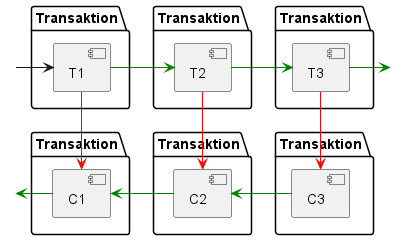
\includegraphics[height=3cm]{figures/ChapterSaga/TransactionScopeSaga-0.png}
		\caption{\small Komponentendiagramm Scope einer zentralisierten Saga mit 3 Operationen}
		\label{fig:transactionscope-saga2}
	\end{minipage}
	\begin{minipage}{.45\textwidth}
		\centering
		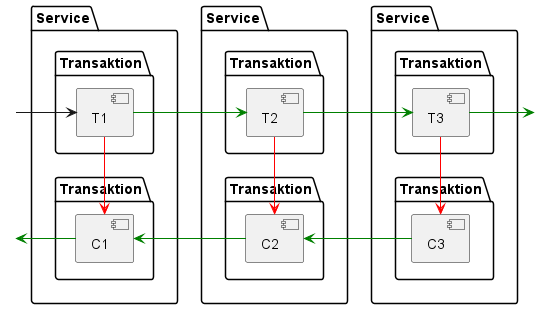
\includegraphics[height=3cm]{figures/ChapterSaga/TransactionScopeDistributedSaga-0.png}
		\caption{\small Komponentendiagramm Scope einer verteilten Transaktion mit 3 Operationen}
		\label{fig:transactionscope-distributed}
	\end{minipage}\hspace{\fill}
\end{figure}
\FloatBarrier
